
% Default to the notebook output style

    


% Inherit from the specified cell style.




    
\documentclass[11pt]{article}

    
    
    \usepackage[T1]{fontenc}
    % Nicer default font (+ math font) than Computer Modern for most use cases
    \usepackage{mathpazo}

    % Basic figure setup, for now with no caption control since it's done
    % automatically by Pandoc (which extracts ![](path) syntax from Markdown).
    \usepackage{graphicx}
    % We will generate all images so they have a width \maxwidth. This means
    % that they will get their normal width if they fit onto the page, but
    % are scaled down if they would overflow the margins.
    \makeatletter
    \def\maxwidth{\ifdim\Gin@nat@width>\linewidth\linewidth
    \else\Gin@nat@width\fi}
    \makeatother
    \let\Oldincludegraphics\includegraphics
    % Set max figure width to be 80% of text width, for now hardcoded.
    \renewcommand{\includegraphics}[1]{\Oldincludegraphics[width=.8\maxwidth]{#1}}
    % Ensure that by default, figures have no caption (until we provide a
    % proper Figure object with a Caption API and a way to capture that
    % in the conversion process - todo).
    \usepackage{caption}
    \DeclareCaptionLabelFormat{nolabel}{}
    \captionsetup{labelformat=nolabel}

    \usepackage{adjustbox} % Used to constrain images to a maximum size 
    \usepackage{xcolor} % Allow colors to be defined
    \usepackage{enumerate} % Needed for markdown enumerations to work
    \usepackage{geometry} % Used to adjust the document margins
    \usepackage{amsmath} % Equations
    \usepackage{amssymb} % Equations
    \usepackage{textcomp} % defines textquotesingle
    % Hack from http://tex.stackexchange.com/a/47451/13684:
    \AtBeginDocument{%
        \def\PYZsq{\textquotesingle}% Upright quotes in Pygmentized code
    }
    \usepackage{upquote} % Upright quotes for verbatim code
    \usepackage{eurosym} % defines \euro
    \usepackage[mathletters]{ucs} % Extended unicode (utf-8) support
    \usepackage[utf8x]{inputenc} % Allow utf-8 characters in the tex document
    \usepackage{fancyvrb} % verbatim replacement that allows latex
    \usepackage{grffile} % extends the file name processing of package graphics 
                         % to support a larger range 
    % The hyperref package gives us a pdf with properly built
    % internal navigation ('pdf bookmarks' for the table of contents,
    % internal cross-reference links, web links for URLs, etc.)
    \usepackage{hyperref}
    \usepackage{longtable} % longtable support required by pandoc >1.10
    \usepackage{booktabs}  % table support for pandoc > 1.12.2
    \usepackage[inline]{enumitem} % IRkernel/repr support (it uses the enumerate* environment)
    \usepackage[normalem]{ulem} % ulem is needed to support strikethroughs (\sout)
                                % normalem makes italics be italics, not underlines
    \usepackage{mathrsfs}
    

    
    
    % Colors for the hyperref package
    \definecolor{urlcolor}{rgb}{0,.145,.698}
    \definecolor{linkcolor}{rgb}{.71,0.21,0.01}
    \definecolor{citecolor}{rgb}{.12,.54,.11}

    % ANSI colors
    \definecolor{ansi-black}{HTML}{3E424D}
    \definecolor{ansi-black-intense}{HTML}{282C36}
    \definecolor{ansi-red}{HTML}{E75C58}
    \definecolor{ansi-red-intense}{HTML}{B22B31}
    \definecolor{ansi-green}{HTML}{00A250}
    \definecolor{ansi-green-intense}{HTML}{007427}
    \definecolor{ansi-yellow}{HTML}{DDB62B}
    \definecolor{ansi-yellow-intense}{HTML}{B27D12}
    \definecolor{ansi-blue}{HTML}{208FFB}
    \definecolor{ansi-blue-intense}{HTML}{0065CA}
    \definecolor{ansi-magenta}{HTML}{D160C4}
    \definecolor{ansi-magenta-intense}{HTML}{A03196}
    \definecolor{ansi-cyan}{HTML}{60C6C8}
    \definecolor{ansi-cyan-intense}{HTML}{258F8F}
    \definecolor{ansi-white}{HTML}{C5C1B4}
    \definecolor{ansi-white-intense}{HTML}{A1A6B2}
    \definecolor{ansi-default-inverse-fg}{HTML}{FFFFFF}
    \definecolor{ansi-default-inverse-bg}{HTML}{000000}

    % commands and environments needed by pandoc snippets
    % extracted from the output of `pandoc -s`
    \providecommand{\tightlist}{%
      \setlength{\itemsep}{0pt}\setlength{\parskip}{0pt}}
    \DefineVerbatimEnvironment{Highlighting}{Verbatim}{commandchars=\\\{\}}
    % Add ',fontsize=\small' for more characters per line
    \newenvironment{Shaded}{}{}
    \newcommand{\KeywordTok}[1]{\textcolor[rgb]{0.00,0.44,0.13}{\textbf{{#1}}}}
    \newcommand{\DataTypeTok}[1]{\textcolor[rgb]{0.56,0.13,0.00}{{#1}}}
    \newcommand{\DecValTok}[1]{\textcolor[rgb]{0.25,0.63,0.44}{{#1}}}
    \newcommand{\BaseNTok}[1]{\textcolor[rgb]{0.25,0.63,0.44}{{#1}}}
    \newcommand{\FloatTok}[1]{\textcolor[rgb]{0.25,0.63,0.44}{{#1}}}
    \newcommand{\CharTok}[1]{\textcolor[rgb]{0.25,0.44,0.63}{{#1}}}
    \newcommand{\StringTok}[1]{\textcolor[rgb]{0.25,0.44,0.63}{{#1}}}
    \newcommand{\CommentTok}[1]{\textcolor[rgb]{0.38,0.63,0.69}{\textit{{#1}}}}
    \newcommand{\OtherTok}[1]{\textcolor[rgb]{0.00,0.44,0.13}{{#1}}}
    \newcommand{\AlertTok}[1]{\textcolor[rgb]{1.00,0.00,0.00}{\textbf{{#1}}}}
    \newcommand{\FunctionTok}[1]{\textcolor[rgb]{0.02,0.16,0.49}{{#1}}}
    \newcommand{\RegionMarkerTok}[1]{{#1}}
    \newcommand{\ErrorTok}[1]{\textcolor[rgb]{1.00,0.00,0.00}{\textbf{{#1}}}}
    \newcommand{\NormalTok}[1]{{#1}}
    
    % Additional commands for more recent versions of Pandoc
    \newcommand{\ConstantTok}[1]{\textcolor[rgb]{0.53,0.00,0.00}{{#1}}}
    \newcommand{\SpecialCharTok}[1]{\textcolor[rgb]{0.25,0.44,0.63}{{#1}}}
    \newcommand{\VerbatimStringTok}[1]{\textcolor[rgb]{0.25,0.44,0.63}{{#1}}}
    \newcommand{\SpecialStringTok}[1]{\textcolor[rgb]{0.73,0.40,0.53}{{#1}}}
    \newcommand{\ImportTok}[1]{{#1}}
    \newcommand{\DocumentationTok}[1]{\textcolor[rgb]{0.73,0.13,0.13}{\textit{{#1}}}}
    \newcommand{\AnnotationTok}[1]{\textcolor[rgb]{0.38,0.63,0.69}{\textbf{\textit{{#1}}}}}
    \newcommand{\CommentVarTok}[1]{\textcolor[rgb]{0.38,0.63,0.69}{\textbf{\textit{{#1}}}}}
    \newcommand{\VariableTok}[1]{\textcolor[rgb]{0.10,0.09,0.49}{{#1}}}
    \newcommand{\ControlFlowTok}[1]{\textcolor[rgb]{0.00,0.44,0.13}{\textbf{{#1}}}}
    \newcommand{\OperatorTok}[1]{\textcolor[rgb]{0.40,0.40,0.40}{{#1}}}
    \newcommand{\BuiltInTok}[1]{{#1}}
    \newcommand{\ExtensionTok}[1]{{#1}}
    \newcommand{\PreprocessorTok}[1]{\textcolor[rgb]{0.74,0.48,0.00}{{#1}}}
    \newcommand{\AttributeTok}[1]{\textcolor[rgb]{0.49,0.56,0.16}{{#1}}}
    \newcommand{\InformationTok}[1]{\textcolor[rgb]{0.38,0.63,0.69}{\textbf{\textit{{#1}}}}}
    \newcommand{\WarningTok}[1]{\textcolor[rgb]{0.38,0.63,0.69}{\textbf{\textit{{#1}}}}}
    
    
    % Define a nice break command that doesn't care if a line doesn't already
    % exist.
    \def\br{\hspace*{\fill} \\* }
    % Math Jax compatibility definitions
    \def\gt{>}
    \def\lt{<}
    \let\Oldtex\TeX
    \let\Oldlatex\LaTeX
    \renewcommand{\TeX}{\textrm{\Oldtex}}
    \renewcommand{\LaTeX}{\textrm{\Oldlatex}}
    % Document parameters
    % Document title
    \title{relazione}
    
    
    
    
    

    % Pygments definitions
    
\makeatletter
\def\PY@reset{\let\PY@it=\relax \let\PY@bf=\relax%
    \let\PY@ul=\relax \let\PY@tc=\relax%
    \let\PY@bc=\relax \let\PY@ff=\relax}
\def\PY@tok#1{\csname PY@tok@#1\endcsname}
\def\PY@toks#1+{\ifx\relax#1\empty\else%
    \PY@tok{#1}\expandafter\PY@toks\fi}
\def\PY@do#1{\PY@bc{\PY@tc{\PY@ul{%
    \PY@it{\PY@bf{\PY@ff{#1}}}}}}}
\def\PY#1#2{\PY@reset\PY@toks#1+\relax+\PY@do{#2}}

\expandafter\def\csname PY@tok@w\endcsname{\def\PY@tc##1{\textcolor[rgb]{0.73,0.73,0.73}{##1}}}
\expandafter\def\csname PY@tok@c\endcsname{\let\PY@it=\textit\def\PY@tc##1{\textcolor[rgb]{0.25,0.50,0.50}{##1}}}
\expandafter\def\csname PY@tok@cp\endcsname{\def\PY@tc##1{\textcolor[rgb]{0.74,0.48,0.00}{##1}}}
\expandafter\def\csname PY@tok@k\endcsname{\let\PY@bf=\textbf\def\PY@tc##1{\textcolor[rgb]{0.00,0.50,0.00}{##1}}}
\expandafter\def\csname PY@tok@kp\endcsname{\def\PY@tc##1{\textcolor[rgb]{0.00,0.50,0.00}{##1}}}
\expandafter\def\csname PY@tok@kt\endcsname{\def\PY@tc##1{\textcolor[rgb]{0.69,0.00,0.25}{##1}}}
\expandafter\def\csname PY@tok@o\endcsname{\def\PY@tc##1{\textcolor[rgb]{0.40,0.40,0.40}{##1}}}
\expandafter\def\csname PY@tok@ow\endcsname{\let\PY@bf=\textbf\def\PY@tc##1{\textcolor[rgb]{0.67,0.13,1.00}{##1}}}
\expandafter\def\csname PY@tok@nb\endcsname{\def\PY@tc##1{\textcolor[rgb]{0.00,0.50,0.00}{##1}}}
\expandafter\def\csname PY@tok@nf\endcsname{\def\PY@tc##1{\textcolor[rgb]{0.00,0.00,1.00}{##1}}}
\expandafter\def\csname PY@tok@nc\endcsname{\let\PY@bf=\textbf\def\PY@tc##1{\textcolor[rgb]{0.00,0.00,1.00}{##1}}}
\expandafter\def\csname PY@tok@nn\endcsname{\let\PY@bf=\textbf\def\PY@tc##1{\textcolor[rgb]{0.00,0.00,1.00}{##1}}}
\expandafter\def\csname PY@tok@ne\endcsname{\let\PY@bf=\textbf\def\PY@tc##1{\textcolor[rgb]{0.82,0.25,0.23}{##1}}}
\expandafter\def\csname PY@tok@nv\endcsname{\def\PY@tc##1{\textcolor[rgb]{0.10,0.09,0.49}{##1}}}
\expandafter\def\csname PY@tok@no\endcsname{\def\PY@tc##1{\textcolor[rgb]{0.53,0.00,0.00}{##1}}}
\expandafter\def\csname PY@tok@nl\endcsname{\def\PY@tc##1{\textcolor[rgb]{0.63,0.63,0.00}{##1}}}
\expandafter\def\csname PY@tok@ni\endcsname{\let\PY@bf=\textbf\def\PY@tc##1{\textcolor[rgb]{0.60,0.60,0.60}{##1}}}
\expandafter\def\csname PY@tok@na\endcsname{\def\PY@tc##1{\textcolor[rgb]{0.49,0.56,0.16}{##1}}}
\expandafter\def\csname PY@tok@nt\endcsname{\let\PY@bf=\textbf\def\PY@tc##1{\textcolor[rgb]{0.00,0.50,0.00}{##1}}}
\expandafter\def\csname PY@tok@nd\endcsname{\def\PY@tc##1{\textcolor[rgb]{0.67,0.13,1.00}{##1}}}
\expandafter\def\csname PY@tok@s\endcsname{\def\PY@tc##1{\textcolor[rgb]{0.73,0.13,0.13}{##1}}}
\expandafter\def\csname PY@tok@sd\endcsname{\let\PY@it=\textit\def\PY@tc##1{\textcolor[rgb]{0.73,0.13,0.13}{##1}}}
\expandafter\def\csname PY@tok@si\endcsname{\let\PY@bf=\textbf\def\PY@tc##1{\textcolor[rgb]{0.73,0.40,0.53}{##1}}}
\expandafter\def\csname PY@tok@se\endcsname{\let\PY@bf=\textbf\def\PY@tc##1{\textcolor[rgb]{0.73,0.40,0.13}{##1}}}
\expandafter\def\csname PY@tok@sr\endcsname{\def\PY@tc##1{\textcolor[rgb]{0.73,0.40,0.53}{##1}}}
\expandafter\def\csname PY@tok@ss\endcsname{\def\PY@tc##1{\textcolor[rgb]{0.10,0.09,0.49}{##1}}}
\expandafter\def\csname PY@tok@sx\endcsname{\def\PY@tc##1{\textcolor[rgb]{0.00,0.50,0.00}{##1}}}
\expandafter\def\csname PY@tok@m\endcsname{\def\PY@tc##1{\textcolor[rgb]{0.40,0.40,0.40}{##1}}}
\expandafter\def\csname PY@tok@gh\endcsname{\let\PY@bf=\textbf\def\PY@tc##1{\textcolor[rgb]{0.00,0.00,0.50}{##1}}}
\expandafter\def\csname PY@tok@gu\endcsname{\let\PY@bf=\textbf\def\PY@tc##1{\textcolor[rgb]{0.50,0.00,0.50}{##1}}}
\expandafter\def\csname PY@tok@gd\endcsname{\def\PY@tc##1{\textcolor[rgb]{0.63,0.00,0.00}{##1}}}
\expandafter\def\csname PY@tok@gi\endcsname{\def\PY@tc##1{\textcolor[rgb]{0.00,0.63,0.00}{##1}}}
\expandafter\def\csname PY@tok@gr\endcsname{\def\PY@tc##1{\textcolor[rgb]{1.00,0.00,0.00}{##1}}}
\expandafter\def\csname PY@tok@ge\endcsname{\let\PY@it=\textit}
\expandafter\def\csname PY@tok@gs\endcsname{\let\PY@bf=\textbf}
\expandafter\def\csname PY@tok@gp\endcsname{\let\PY@bf=\textbf\def\PY@tc##1{\textcolor[rgb]{0.00,0.00,0.50}{##1}}}
\expandafter\def\csname PY@tok@go\endcsname{\def\PY@tc##1{\textcolor[rgb]{0.53,0.53,0.53}{##1}}}
\expandafter\def\csname PY@tok@gt\endcsname{\def\PY@tc##1{\textcolor[rgb]{0.00,0.27,0.87}{##1}}}
\expandafter\def\csname PY@tok@err\endcsname{\def\PY@bc##1{\setlength{\fboxsep}{0pt}\fcolorbox[rgb]{1.00,0.00,0.00}{1,1,1}{\strut ##1}}}
\expandafter\def\csname PY@tok@kc\endcsname{\let\PY@bf=\textbf\def\PY@tc##1{\textcolor[rgb]{0.00,0.50,0.00}{##1}}}
\expandafter\def\csname PY@tok@kd\endcsname{\let\PY@bf=\textbf\def\PY@tc##1{\textcolor[rgb]{0.00,0.50,0.00}{##1}}}
\expandafter\def\csname PY@tok@kn\endcsname{\let\PY@bf=\textbf\def\PY@tc##1{\textcolor[rgb]{0.00,0.50,0.00}{##1}}}
\expandafter\def\csname PY@tok@kr\endcsname{\let\PY@bf=\textbf\def\PY@tc##1{\textcolor[rgb]{0.00,0.50,0.00}{##1}}}
\expandafter\def\csname PY@tok@bp\endcsname{\def\PY@tc##1{\textcolor[rgb]{0.00,0.50,0.00}{##1}}}
\expandafter\def\csname PY@tok@fm\endcsname{\def\PY@tc##1{\textcolor[rgb]{0.00,0.00,1.00}{##1}}}
\expandafter\def\csname PY@tok@vc\endcsname{\def\PY@tc##1{\textcolor[rgb]{0.10,0.09,0.49}{##1}}}
\expandafter\def\csname PY@tok@vg\endcsname{\def\PY@tc##1{\textcolor[rgb]{0.10,0.09,0.49}{##1}}}
\expandafter\def\csname PY@tok@vi\endcsname{\def\PY@tc##1{\textcolor[rgb]{0.10,0.09,0.49}{##1}}}
\expandafter\def\csname PY@tok@vm\endcsname{\def\PY@tc##1{\textcolor[rgb]{0.10,0.09,0.49}{##1}}}
\expandafter\def\csname PY@tok@sa\endcsname{\def\PY@tc##1{\textcolor[rgb]{0.73,0.13,0.13}{##1}}}
\expandafter\def\csname PY@tok@sb\endcsname{\def\PY@tc##1{\textcolor[rgb]{0.73,0.13,0.13}{##1}}}
\expandafter\def\csname PY@tok@sc\endcsname{\def\PY@tc##1{\textcolor[rgb]{0.73,0.13,0.13}{##1}}}
\expandafter\def\csname PY@tok@dl\endcsname{\def\PY@tc##1{\textcolor[rgb]{0.73,0.13,0.13}{##1}}}
\expandafter\def\csname PY@tok@s2\endcsname{\def\PY@tc##1{\textcolor[rgb]{0.73,0.13,0.13}{##1}}}
\expandafter\def\csname PY@tok@sh\endcsname{\def\PY@tc##1{\textcolor[rgb]{0.73,0.13,0.13}{##1}}}
\expandafter\def\csname PY@tok@s1\endcsname{\def\PY@tc##1{\textcolor[rgb]{0.73,0.13,0.13}{##1}}}
\expandafter\def\csname PY@tok@mb\endcsname{\def\PY@tc##1{\textcolor[rgb]{0.40,0.40,0.40}{##1}}}
\expandafter\def\csname PY@tok@mf\endcsname{\def\PY@tc##1{\textcolor[rgb]{0.40,0.40,0.40}{##1}}}
\expandafter\def\csname PY@tok@mh\endcsname{\def\PY@tc##1{\textcolor[rgb]{0.40,0.40,0.40}{##1}}}
\expandafter\def\csname PY@tok@mi\endcsname{\def\PY@tc##1{\textcolor[rgb]{0.40,0.40,0.40}{##1}}}
\expandafter\def\csname PY@tok@il\endcsname{\def\PY@tc##1{\textcolor[rgb]{0.40,0.40,0.40}{##1}}}
\expandafter\def\csname PY@tok@mo\endcsname{\def\PY@tc##1{\textcolor[rgb]{0.40,0.40,0.40}{##1}}}
\expandafter\def\csname PY@tok@ch\endcsname{\let\PY@it=\textit\def\PY@tc##1{\textcolor[rgb]{0.25,0.50,0.50}{##1}}}
\expandafter\def\csname PY@tok@cm\endcsname{\let\PY@it=\textit\def\PY@tc##1{\textcolor[rgb]{0.25,0.50,0.50}{##1}}}
\expandafter\def\csname PY@tok@cpf\endcsname{\let\PY@it=\textit\def\PY@tc##1{\textcolor[rgb]{0.25,0.50,0.50}{##1}}}
\expandafter\def\csname PY@tok@c1\endcsname{\let\PY@it=\textit\def\PY@tc##1{\textcolor[rgb]{0.25,0.50,0.50}{##1}}}
\expandafter\def\csname PY@tok@cs\endcsname{\let\PY@it=\textit\def\PY@tc##1{\textcolor[rgb]{0.25,0.50,0.50}{##1}}}

\def\PYZbs{\char`\\}
\def\PYZus{\char`\_}
\def\PYZob{\char`\{}
\def\PYZcb{\char`\}}
\def\PYZca{\char`\^}
\def\PYZam{\char`\&}
\def\PYZlt{\char`\<}
\def\PYZgt{\char`\>}
\def\PYZsh{\char`\#}
\def\PYZpc{\char`\%}
\def\PYZdl{\char`\$}
\def\PYZhy{\char`\-}
\def\PYZsq{\char`\'}
\def\PYZdq{\char`\"}
\def\PYZti{\char`\~}
% for compatibility with earlier versions
\def\PYZat{@}
\def\PYZlb{[}
\def\PYZrb{]}
\makeatother


    % Exact colors from NB
    \definecolor{incolor}{rgb}{0.0, 0.0, 0.5}
    \definecolor{outcolor}{rgb}{0.545, 0.0, 0.0}



    
    % Prevent overflowing lines due to hard-to-break entities
    \sloppy 
    % Setup hyperref package
    \hypersetup{
      breaklinks=true,  % so long urls are correctly broken across lines
      colorlinks=true,
      urlcolor=urlcolor,
      linkcolor=linkcolor,
      citecolor=citecolor,
      }
    % Slightly bigger margins than the latex defaults
    
    \geometry{verbose,tmargin=1in,bmargin=1in,lmargin=1in,rmargin=1in}
    
    

    \begin{document}
    
    
    \maketitle
    
    

    
    \hypertarget{verifica-della-legge-dellinverso-del-quadrato-per-lintensituxe0-luminosa}{%
\section{Verifica della legge dell'inverso del quadrato per l'intensità
luminosa}\label{verifica-della-legge-dellinverso-del-quadrato-per-lintensituxe0-luminosa}}

    \hypertarget{motivazione}{%
\subsection{Motivazione}\label{motivazione}}

Data una sorgente luminosa puntiforme \(S\), la teoria fornisce il
valore dell'intensità luminosa \(I\) in un punto \(P\) a distanza
\(r=\overline{PS}\) dalla sorgente attraverso la relazione
\[I=\frac{P}{4\pi r^2}\propto \frac{1}{r^2},\] dove
\(P=\frac{\delta E}{\delta t}\) è la potenza erogata dalla sorgente.

Si vuole verificare sperimentalmente la dipendenza dell'intensità
luminosa dall'inverso del quadrato della distanza utilizzando sensori di
distanza e luminosità collegati ad un software di analisi dati
attraverso la piattaforma \href{https://www.arduino.cc/}{arduino}.

    \hypertarget{strumentazione}{%
\subsection{Strumentazione}\label{strumentazione}}

\begin{itemize}
\tightlist
\item
  Arduino UNO
\item
  Sensore di luminosità (LDR)
  (\href{https://cdn-learn.adafruit.com/downloads/pdf/photocells.pdf}{datasheet})
\item
  Sensore di distanza ad ultrasuoni HC-SR04
  (\href{https://www.electroschematics.com/wp-content/uploads/2013/07/HCSR04-datasheet-version-1.pdf}{datasheet})
\item
  LED RGB
\item
  Batteria al litio da \(3\:V\)
\end{itemize}

    \hypertarget{setup-sperimentale}{%
\subsection{Setup sperimentale}\label{setup-sperimentale}}

Una buona sorgente luminosa puntiforme omnidirezionale può essere
ottenuta alimentando un LED (meglio se verde) con una batteria al litio
da \(3\: V\). Il LED deve essere inserito all'interno di un cartoncino
nero (come in figura) al fine di poter misurare contemporaneamente
intensità luminosa e distanza dalla sorgente. Naturalmente,
l'esperimento va eseguito in condizioni di buio ambientale.

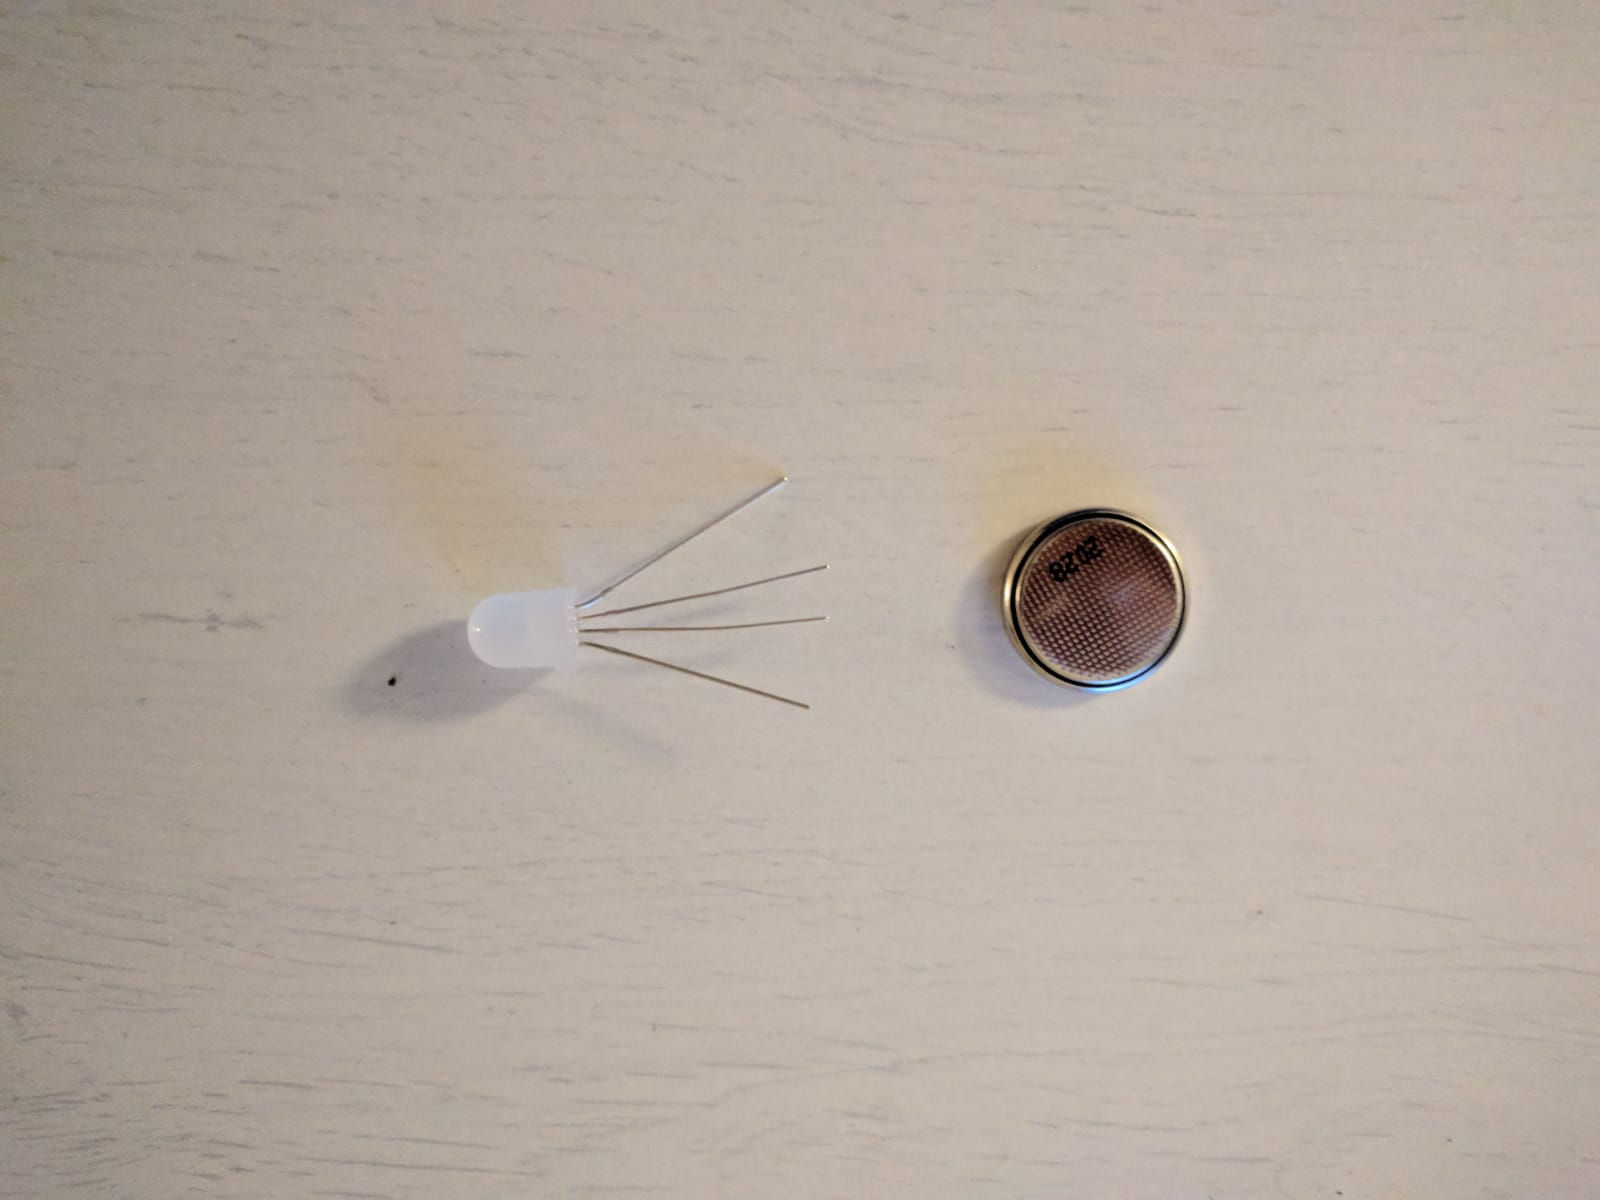
\includegraphics{led.jpeg} 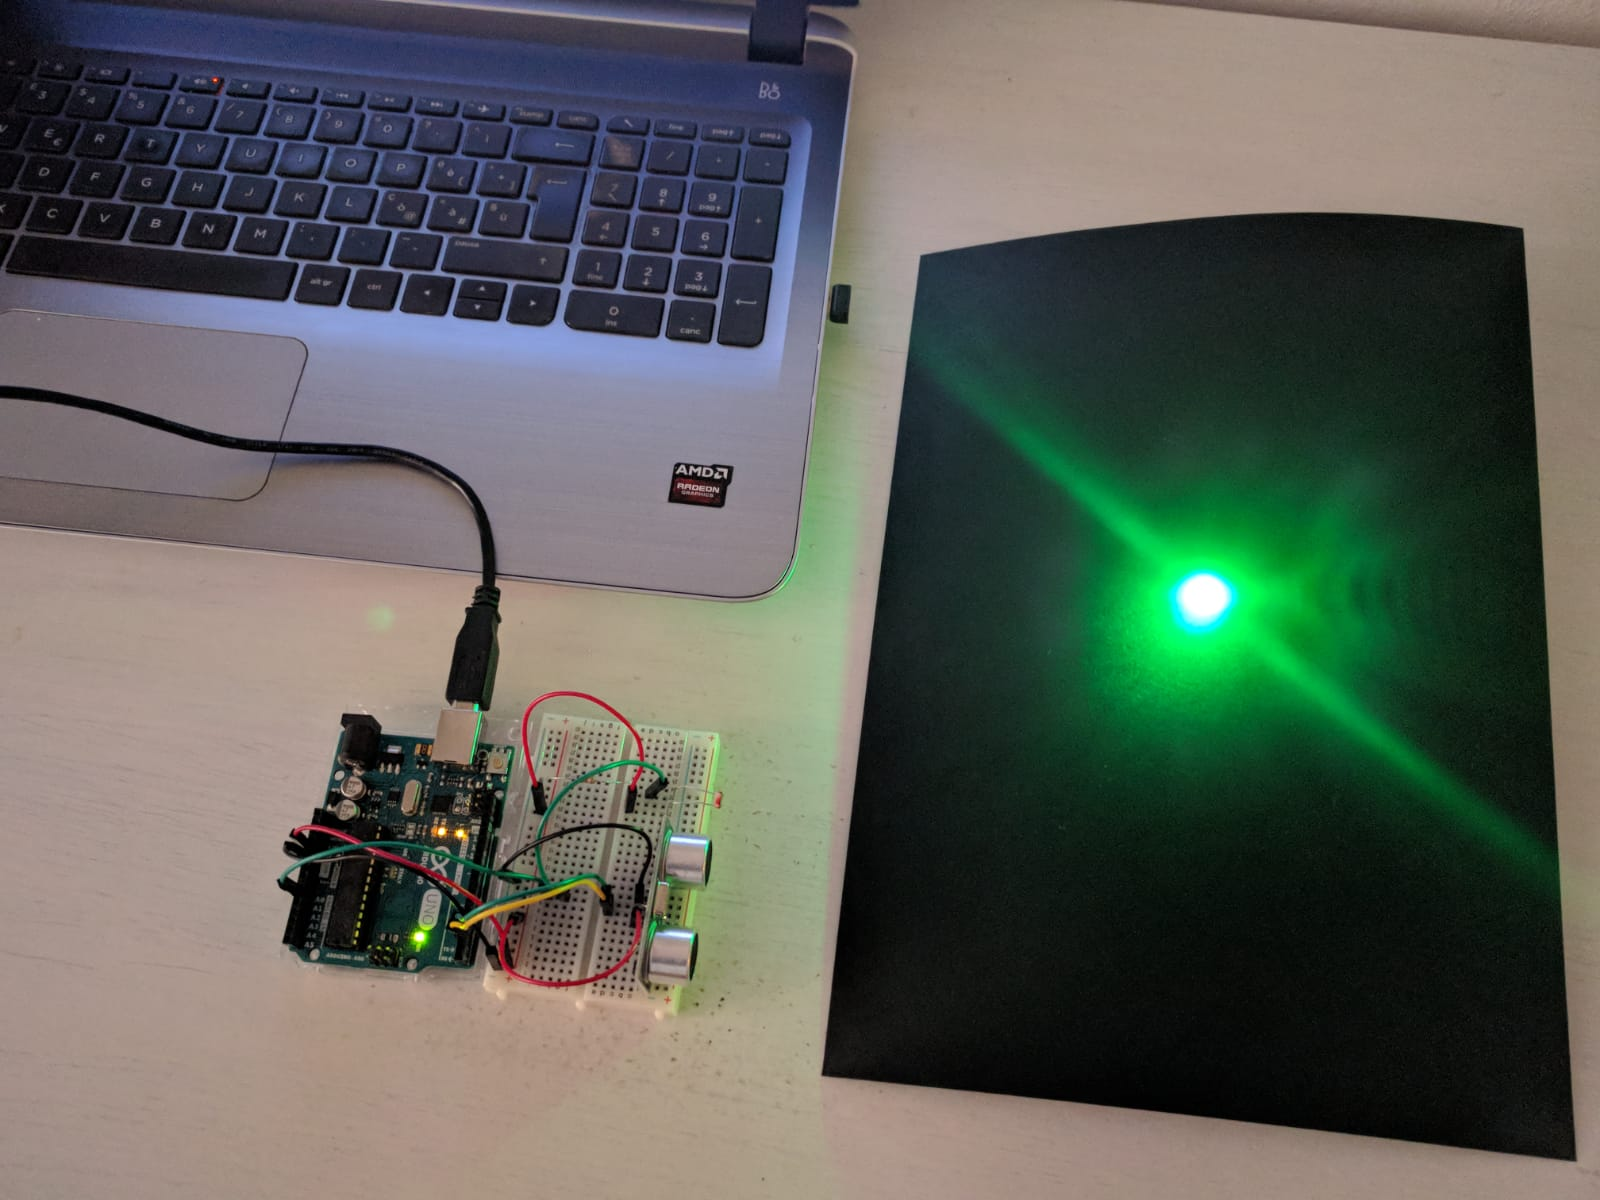
\includegraphics{setup.jpeg}

\hypertarget{schema-del-circuito}{%
\subsubsection{Schema del circuito}\label{schema-del-circuito}}

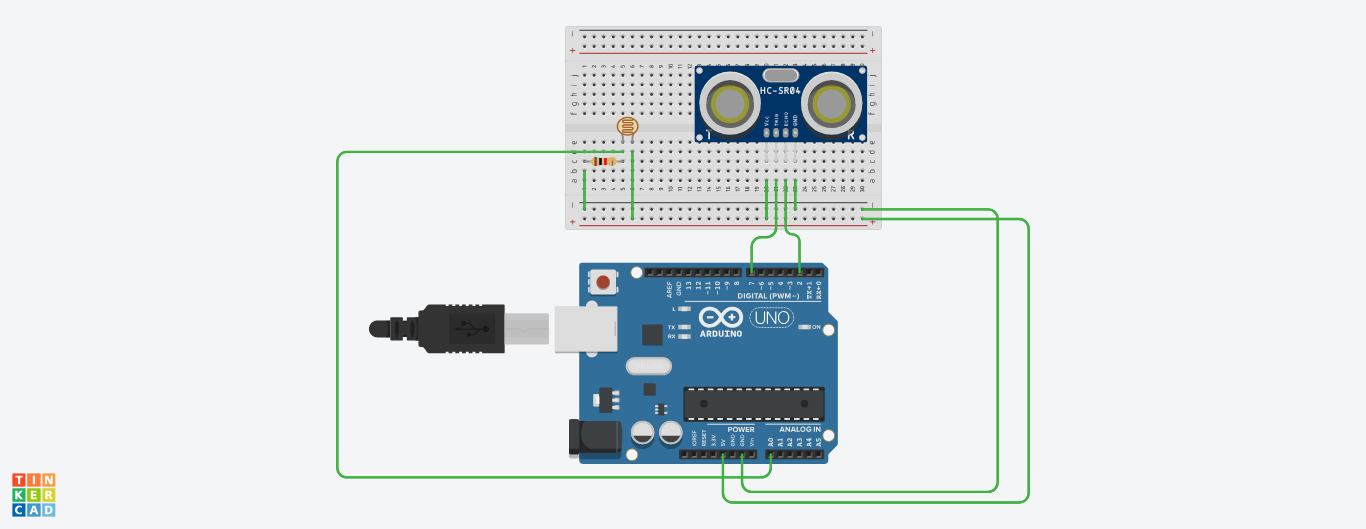
\includegraphics{schema.png} 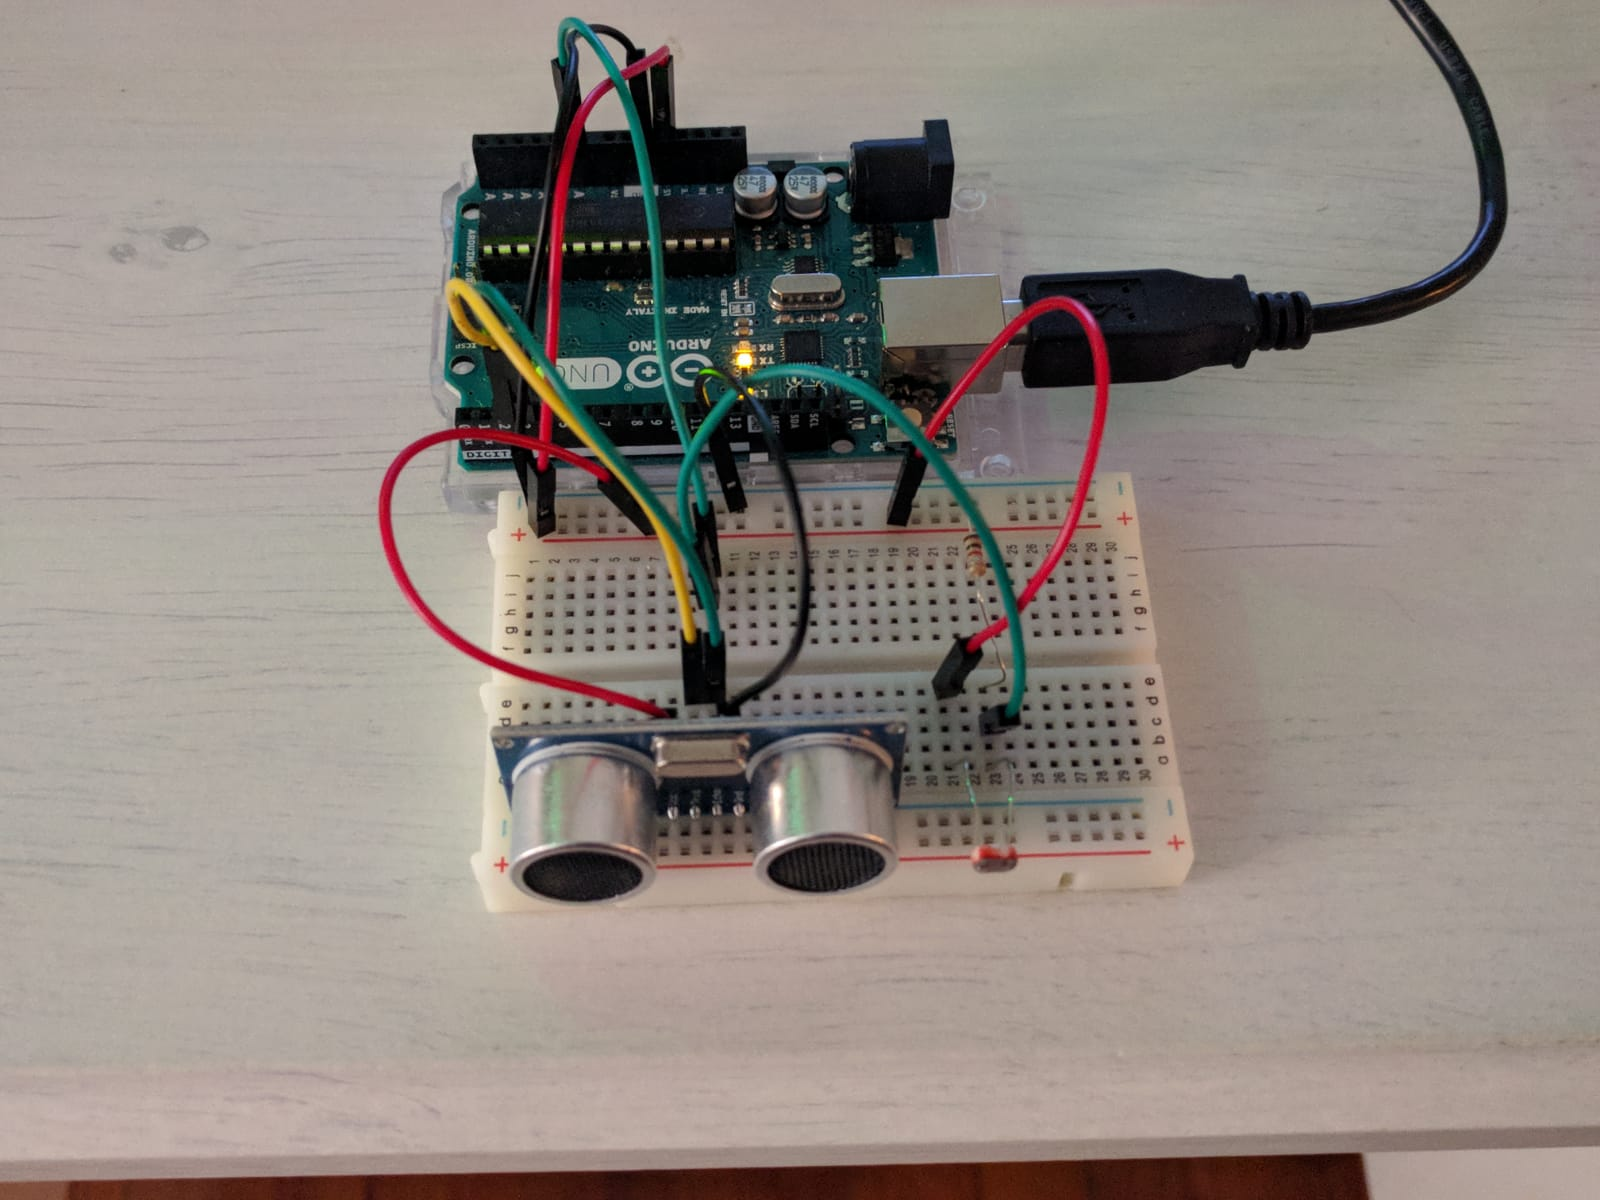
\includegraphics{arduino.jpeg}

\hypertarget{sensore-di-luminosituxe0}{%
\subsubsection{Sensore di luminosità}\label{sensore-di-luminosituxe0}}

La luminosità, a cui è sensibile la fotoresistenza \(R_x\), viene
determinata dalla lettura del potenziale \(V\) fra la fotoresistenza ed
un resistore \(R\) da \(10\:k\Omega\) in serie. Uguagliando le correnti
che attraversano \(R\) ed \(R_x\) abbiamo
\[\frac{V}{R}=\frac{\varepsilon-V}{R_x},\] dove \(\varepsilon=5\:V\) è
la tensione fornita al circuito dalla scheda Arduino UNO. Ne segue che
\[R_x\propto \frac{\varepsilon-V}{V}.\] In base alle specifiche della
fotoresistenza si può considerare una proporzionalità inversa fra
intensità luminosa \(I\) e resistenza \(R_x\) della fotocella. Si può
dunque concludere che \[I\propto \frac{V}{\varepsilon-V}.\] La grandezza
misurata sarà quindi l'intensità adimensionale
\[\frac{I}{I_0}=\frac{V}{\varepsilon-V},\] dove \(I_0\) è l'intensità
corrispondente ad una tensione \(V=\frac{1}{2}\varepsilon=2.5\:V\) e il
cui valore non ha particolare interesse ai fini dell'esperimento.

Per quanto riguarda l'incertezza dell'intensità misurata possiamo
assumere un'incertezza unitaria \(\delta y\) sulla lettura digitale
\(y\) sul pin A0 e propagare l'errore su \(\frac{I}{I_0}\). Considerato
che \(V=cy\) con \(c=\frac{5.0}{1023}\:V\), otteniamo
\[\delta\left(\frac{I}{I_0}\right)=\frac{\partial}{\partial y}\left(\frac{cy}{\varepsilon-cy}\right)\delta y=\frac{c\varepsilon}{(\varepsilon-V)^2}.\]

\hypertarget{sensore-di-distanza-ad-ultrasuoni}{%
\subsubsection{Sensore di distanza ad
ultrasuoni}\label{sensore-di-distanza-ad-ultrasuoni}}

In base alle specifiche del sensore HC-SR04 si può considerare
l'incertezza sulle misure di distanza pari a \(\delta r=0.3\: cm\).

    \hypertarget{codice-arduino}{%
\subsection{Codice arduino}\label{codice-arduino}}

Il codice caricato sull'arduino UNO è il seguente.

\begin{Shaded}
\begin{Highlighting}[]
\DataTypeTok{int}\NormalTok{ photocellPin = A0;}
\DataTypeTok{int}\NormalTok{ triggerPin = }\DecValTok{2}\NormalTok{;}
\DataTypeTok{int}\NormalTok{ echoPin = }\DecValTok{3}\NormalTok{;}

\DataTypeTok{float}\NormalTok{ speedOfSound = }\FloatTok{0.034}\NormalTok{; }\CommentTok{// cm / microseconds}

\DataTypeTok{void}\NormalTok{ setup() \{}
\NormalTok{  pinMode(triggerPin, OUTPUT);}
\NormalTok{  pinMode(echoPin, INPUT);}
\NormalTok{  Serial.begin(}\DecValTok{9600}\NormalTok{);}
\NormalTok{\}}

\DataTypeTok{void}\NormalTok{ loop() \{}
  \DataTypeTok{float}\NormalTok{ t = millis() / }\FloatTok{1000.0}\NormalTok{; }\CommentTok{// secondi dall'avvio del programma}
  \DataTypeTok{int}\NormalTok{ photocellValue = analogRead(photocellPin); }\CommentTok{// lettura della fotoresistenza}
  \DataTypeTok{float}\NormalTok{ V = photocellValue * }\FloatTok{5.0}\NormalTok{ / }\FloatTok{1023.0}\NormalTok{; }\CommentTok{// conversione in tensione}
  \DataTypeTok{float}\NormalTok{ intensity = V / (}\FloatTok{5.0}\NormalTok{ - V); }\CommentTok{// conversione in intensità adimensionale}
  \DataTypeTok{float}\NormalTok{ intensity_err = }\FloatTok{5.0}\NormalTok{ * }\FloatTok{5.0}\NormalTok{ / }\FloatTok{1023.0}\NormalTok{ / ((}\FloatTok{5.0}\NormalTok{ - V) * (}\FloatTok{5.0}\NormalTok{ - V)); }\CommentTok{// calcolo dell'incertezza sull'intensità}
\NormalTok{  digitalWrite(triggerPin, LOW);}
\NormalTok{  digitalWrite(triggerPin, HIGH);}
\NormalTok{  delayMicroseconds(}\DecValTok{10}\NormalTok{);}
\NormalTok{  digitalWrite(triggerPin, LOW);}
  \DataTypeTok{float}\NormalTok{ dt = pulseIn(echoPin, HIGH); }\CommentTok{// lettura del tempo di andata e ritorno del segnale}
  \DataTypeTok{float}\NormalTok{ distance = speedOfSound * dt / }\DecValTok{2}\NormalTok{; }\CommentTok{// calcolo della distanza}
  \DataTypeTok{float}\NormalTok{ distance_err = }\FloatTok{0.3}\NormalTok{; }\CommentTok{// incertezza sulla misura di distanza}
  \ControlFlowTok{if}\NormalTok{ (distance > }\DecValTok{2}\NormalTok{ && distance < }\DecValTok{400}\NormalTok{) \{ }\CommentTok{// controllo che il valore sia nel range di sensibilità}
\NormalTok{    Serial.print(t);}
\NormalTok{    Serial.print(}\StringTok{" "}\NormalTok{);}
\NormalTok{    Serial.print(distance, }\DecValTok{1}\NormalTok{);}
\NormalTok{    Serial.print(}\StringTok{" "}\NormalTok{);}
\NormalTok{    Serial.print(distance_err, }\DecValTok{1}\NormalTok{);}
\NormalTok{    Serial.print(}\StringTok{" "}\NormalTok{);}
\NormalTok{    Serial.print(intensity, }\DecValTok{4}\NormalTok{);}
\NormalTok{    Serial.print(}\StringTok{" "}\NormalTok{);}
\NormalTok{    Serial.println(intensity_err, }\DecValTok{4}\NormalTok{);}
\NormalTok{  \}}
\NormalTok{  delay(}\DecValTok{300}\NormalTok{);}
\NormalTok{\}}
\end{Highlighting}
\end{Shaded}

    \hypertarget{python}{%
\subsection{Python}\label{python}}

Al fine di analizzare adeguatamente i dati è necessario del software
aggiuntivo. Il linguaggio python consente di interfacciarsi con arduino
attraverso una porta seriale.

\hypertarget{installazione}{%
\subsubsection{Installazione}\label{installazione}}

Il software python si trova alla pagina
https://www.python.org/downloads/ (durante l'installazione spuntare la
voce \texttt{Add\ to\ Path}). Una volta installato python è necessario
installare alcune librerie aggiuntive. Aprire dunque il terminale e
inserire il comando

\begin{Shaded}
\begin{Highlighting}[]
\ExtensionTok{pip}\NormalTok{ install pyserial numpy matplotlib jupyter-notebook}
\end{Highlighting}
\end{Shaded}

\hypertarget{modalituxe0-di-acquisizione-dati}{%
\subsubsection{Modalità di acquisizione
dati}\label{modalituxe0-di-acquisizione-dati}}

I dati possono essere acquisiti in diversi modi: - Plotting in
real-time: eseguire il programma \texttt{plotter.py} attraverso il
comando da terminale (verificare che la porta di arduino sia
\texttt{COM3} o modificare il programma)

\begin{Shaded}
\begin{Highlighting}[]
\ExtensionTok{python}\NormalTok{ plotter.py}
\end{Highlighting}
\end{Shaded}

\begin{itemize}
\tightlist
\item
  Esportazione per foglio di calcolo: eseguire il programma
  \texttt{arduino2excel.py} attraverso il comando da terminale
  (verificare che la porta di arduino sia \texttt{COM3} o modificare il
  programma)
\end{itemize}

\begin{Shaded}
\begin{Highlighting}[]
\ExtensionTok{python}\NormalTok{ arduino2excel.py}
\end{Highlighting}
\end{Shaded}

\begin{itemize}
\tightlist
\item
  Jupyter notebook: eseguire il comando da terminale
\end{itemize}

\begin{Shaded}
\begin{Highlighting}[]
\ExtensionTok{jupyter}\NormalTok{ notebook relazione.ipynb}
\end{Highlighting}
\end{Shaded}

    \hypertarget{acquisizione-dati}{%
\subsection{Acquisizione dati}\label{acquisizione-dati}}

Importiamo le librerie necessarie: - \texttt{serial} per la
comunicazione arduino-computer, - \texttt{matplotlib} per il plotting
dei dati, - \texttt{numpy} per la manipolazione numerica dei dati.

    \begin{Verbatim}[commandchars=\\\{\}]
{\color{incolor}In [{\color{incolor}1}]:} \PY{o}{\PYZpc{}}\PY{k}{matplotlib} notebook
        
        \PY{k+kn}{import} \PY{n+nn}{serial}
        \PY{k+kn}{import} \PY{n+nn}{matplotlib}\PY{n+nn}{.}\PY{n+nn}{pyplot} \PY{k}{as} \PY{n+nn}{plt}
        \PY{k+kn}{import} \PY{n+nn}{numpy} \PY{k}{as} \PY{n+nn}{np}
\end{Verbatim}

    Inizializziamo la comunicazione seriale arduino-computer e definiamo
alcune funzioni di utilità. Verificare che la porta di arduino sia
\texttt{COM3} o modificare opportunamente il seguente codice.

    \begin{Verbatim}[commandchars=\\\{\}]
{\color{incolor}In [{\color{incolor}59}]:} \PY{n}{ser} \PY{o}{=} \PY{n}{serial}\PY{o}{.}\PY{n}{Serial}\PY{p}{(}\PY{l+s+s1}{\PYZsq{}}\PY{l+s+s1}{COM3}\PY{l+s+s1}{\PYZsq{}}\PY{p}{)}
         
         \PY{k}{def} \PY{n+nf}{open\PYZus{}serial\PYZus{}comm}\PY{p}{(}\PY{p}{)}\PY{p}{:}
             \PY{k}{global} \PY{n}{ser}
             \PY{k}{if} \PY{o+ow}{not} \PY{n}{ser}\PY{o}{.}\PY{n}{is\PYZus{}open}\PY{p}{:}
                 \PY{n}{ser}\PY{o}{.}\PY{n}{open}\PY{p}{(}\PY{p}{)}
         
         \PY{k}{def} \PY{n+nf}{close\PYZus{}serial\PYZus{}comm}\PY{p}{(}\PY{p}{)}\PY{p}{:}
             \PY{k}{global} \PY{n}{ser}
             \PY{k}{if} \PY{n}{ser}\PY{o}{.}\PY{n}{is\PYZus{}open}\PY{p}{:}
                 \PY{n}{ser}\PY{o}{.}\PY{n}{close}\PY{p}{(}\PY{p}{)}
                 
         \PY{k}{def} \PY{n+nf}{read\PYZus{}serial\PYZus{}data}\PY{p}{(}\PY{p}{)}\PY{p}{:}
             \PY{k}{global} \PY{n}{ser}
             \PY{n}{raw\PYZus{}data\PYZus{}line} \PY{o}{=} \PY{n}{ser}\PY{o}{.}\PY{n}{readline}\PY{p}{(}\PY{p}{)}\PY{o}{.}\PY{n}{decode}\PY{p}{(}\PY{l+s+s1}{\PYZsq{}}\PY{l+s+s1}{ascii}\PY{l+s+s1}{\PYZsq{}}\PY{p}{)}
             \PY{n}{t}\PY{p}{,} \PY{n}{r}\PY{p}{,} \PY{n}{r\PYZus{}err}\PY{p}{,} \PY{n}{I}\PY{p}{,} \PY{n}{I\PYZus{}err} \PY{o}{=} \PY{n+nb}{list}\PY{p}{(}\PY{n+nb}{map}\PY{p}{(}\PY{k}{lambda} \PY{n}{x}\PY{p}{:} \PY{n+nb}{float}\PY{p}{(}\PY{n}{x}\PY{p}{)}\PY{p}{,} \PY{n}{raw\PYZus{}data\PYZus{}line}\PY{o}{.}\PY{n}{split}\PY{p}{(}\PY{l+s+s1}{\PYZsq{}}\PY{l+s+s1}{ }\PY{l+s+s1}{\PYZsq{}}\PY{p}{)}\PY{p}{)}\PY{p}{)}
             \PY{k}{return} \PY{n}{t}\PY{p}{,} \PY{n}{r}\PY{p}{,} \PY{n}{r\PYZus{}err}\PY{p}{,} \PY{n}{I}\PY{p}{,} \PY{n}{I\PYZus{}err}
\end{Verbatim}

    Impostiamo il numero di dati da acquisire e inizializziamo gli array per
le distanze e le intensità.

    \begin{Verbatim}[commandchars=\\\{\}]
{\color{incolor}In [{\color{incolor}83}]:} \PY{n}{N} \PY{o}{=} \PY{l+m+mi}{50} \PY{c+c1}{\PYZsh{} numero dati}
         
         \PY{n}{rs} \PY{o}{=} \PY{n}{np}\PY{o}{.}\PY{n}{empty}\PY{p}{(}\PY{n}{N}\PY{p}{)} \PY{c+c1}{\PYZsh{} array di lunghezza N per le distanze}
         \PY{n}{Is} \PY{o}{=} \PY{n}{np}\PY{o}{.}\PY{n}{empty}\PY{p}{(}\PY{n}{N}\PY{p}{)} \PY{c+c1}{\PYZsh{} array di lunghezza N per le intensità}
         
         \PY{n}{rs\PYZus{}err} \PY{o}{=} \PY{n}{np}\PY{o}{.}\PY{n}{full}\PY{p}{(}\PY{p}{(}\PY{n}{N}\PY{p}{,}\PY{p}{)}\PY{p}{,} \PY{l+m+mf}{0.3}\PY{p}{)} \PY{c+c1}{\PYZsh{} array di lunghezza N per le incertezze sulle distanze}
         \PY{n}{Is\PYZus{}err} \PY{o}{=} \PY{n}{np}\PY{o}{.}\PY{n}{empty}\PY{p}{(}\PY{n}{N}\PY{p}{)} \PY{c+c1}{\PYZsh{} array di lunghezza N per le incertezze sull\PYZsq{}intensità}
\end{Verbatim}

    Acquisiamo i dati attraverso l'interfaccia seriale con Arduino.

    \begin{Verbatim}[commandchars=\\\{\}]
{\color{incolor}In [{\color{incolor}85}]:} \PY{n}{fig} \PY{o}{=} \PY{n}{plt}\PY{o}{.}\PY{n}{figure}\PY{p}{(}\PY{l+s+s1}{\PYZsq{}}\PY{l+s+s1}{Dati}\PY{l+s+s1}{\PYZsq{}}\PY{p}{)}
         \PY{n}{plt}\PY{o}{.}\PY{n}{xlabel}\PY{p}{(}\PY{l+s+sa}{r}\PY{l+s+s1}{\PYZsq{}}\PY{l+s+s1}{\PYZdl{}r}\PY{l+s+s1}{\PYZbs{}}\PY{l+s+s1}{:(cm)\PYZdl{}}\PY{l+s+s1}{\PYZsq{}}\PY{p}{)}
         \PY{n}{plt}\PY{o}{.}\PY{n}{ylabel}\PY{p}{(}\PY{l+s+sa}{r}\PY{l+s+s1}{\PYZsq{}}\PY{l+s+s1}{\PYZdl{}}\PY{l+s+s1}{\PYZbs{}}\PY{l+s+s1}{frac}\PY{l+s+si}{\PYZob{}I\PYZcb{}}\PY{l+s+si}{\PYZob{}I\PYZus{}0\PYZcb{}}\PY{l+s+s1}{\PYZdl{}}\PY{l+s+s1}{\PYZsq{}}\PY{p}{)}
         
         \PY{n}{open\PYZus{}serial\PYZus{}comm}\PY{p}{(}\PY{p}{)}
         
         \PY{k}{for} \PY{n}{i} \PY{o+ow}{in} \PY{n+nb}{range}\PY{p}{(}\PY{n}{N}\PY{p}{)}\PY{p}{:}
             \PY{n}{t}\PY{p}{,} \PY{n}{r}\PY{p}{,} \PY{n}{r\PYZus{}err}\PY{p}{,} \PY{n}{I}\PY{p}{,} \PY{n}{I\PYZus{}err} \PY{o}{=} \PY{n}{read\PYZus{}serial\PYZus{}data}\PY{p}{(}\PY{p}{)}
             \PY{n}{rs}\PY{p}{[}\PY{n}{i}\PY{p}{]}\PY{p}{,} \PY{n}{rs\PYZus{}err}\PY{p}{[}\PY{n}{i}\PY{p}{]}\PY{p}{,} \PY{n}{Is}\PY{p}{[}\PY{n}{i}\PY{p}{]}\PY{p}{,} \PY{n}{Is\PYZus{}err}\PY{p}{[}\PY{n}{i}\PY{p}{]} \PY{o}{=} \PY{n}{r}\PY{p}{,} \PY{n}{r\PYZus{}err}\PY{p}{,} \PY{n}{I}\PY{p}{,} \PY{n}{I\PYZus{}err}
             \PY{n}{plt}\PY{o}{.}\PY{n}{plot}\PY{p}{(}\PY{n}{r}\PY{p}{,} \PY{n}{I}\PY{p}{,} \PY{l+s+s1}{\PYZsq{}}\PY{l+s+s1}{bo}\PY{l+s+s1}{\PYZsq{}}\PY{p}{)}
             \PY{n}{fig}\PY{o}{.}\PY{n}{canvas}\PY{o}{.}\PY{n}{draw}\PY{p}{(}\PY{p}{)}
         
         \PY{n}{close\PYZus{}serial\PYZus{}comm}\PY{p}{(}\PY{p}{)}
\end{Verbatim}

    
    \begin{verbatim}
<IPython.core.display.Javascript object>
    \end{verbatim}

    
    
    \begin{verbatim}
<IPython.core.display.HTML object>
    \end{verbatim}

    
    Riportiamo i dati acquisiti in formato \emph{csv}.

    \begin{Verbatim}[commandchars=\\\{\}]
{\color{incolor}In [{\color{incolor}86}]:} \PY{n+nb}{print}\PY{p}{(}\PY{l+s+s1}{\PYZsq{}}\PY{l+s+s1}{\PYZsh{},}\PY{l+s+se}{\PYZbs{}t}\PY{l+s+s1}{r,}\PY{l+s+se}{\PYZbs{}t}\PY{l+s+s1}{r\PYZus{}err,}\PY{l+s+se}{\PYZbs{}t}\PY{l+s+s1}{I,}\PY{l+s+se}{\PYZbs{}t}\PY{l+s+s1}{I\PYZus{}err}\PY{l+s+s1}{\PYZsq{}}\PY{p}{)}
         \PY{k}{for} \PY{n}{i} \PY{o+ow}{in} \PY{n+nb}{range}\PY{p}{(}\PY{n}{N}\PY{p}{)}\PY{p}{:}
             \PY{n+nb}{print}\PY{p}{(}\PY{n}{f}\PY{l+s+s1}{\PYZsq{}}\PY{l+s+si}{\PYZob{}i\PYZcb{}}\PY{l+s+s1}{,}\PY{l+s+se}{\PYZbs{}t}\PY{l+s+si}{\PYZob{}rs[i]\PYZcb{}}\PY{l+s+s1}{,}\PY{l+s+se}{\PYZbs{}t}\PY{l+s+si}{\PYZob{}rs\PYZus{}err[i]\PYZcb{}}\PY{l+s+s1}{,}\PY{l+s+se}{\PYZbs{}t}\PY{l+s+si}{\PYZob{}Is[i]\PYZcb{}}\PY{l+s+s1}{,}\PY{l+s+se}{\PYZbs{}t}\PY{l+s+si}{\PYZob{}Is\PYZus{}err[i]\PYZcb{}}\PY{l+s+s1}{\PYZsq{}}\PY{p}{)}
\end{Verbatim}

    \begin{Verbatim}[commandchars=\\\{\}]
\#,	r,	r\_err,	I,	I\_err
0,	29.3,	0.3,	0.1048,	0.0012
1,	29.1,	0.3,	0.1059,	0.0012
2,	28.9,	0.3,	0.1083,	0.0012
3,	28.4,	0.3,	0.1095,	0.0012
4,	28.0,	0.3,	0.1107,	0.0012
5,	27.6,	0.3,	0.1144,	0.0012
6,	27.0,	0.3,	0.118,	0.0012
7,	26.5,	0.3,	0.1217,	0.0012
8,	25.7,	0.3,	0.1267,	0.0012
9,	25.1,	0.3,	0.1304,	0.0012
10,	24.5,	0.3,	0.1354,	0.0013
11,	23.9,	0.3,	0.1405,	0.0013
12,	23.2,	0.3,	0.1469,	0.0013
13,	23.2,	0.3,	0.1507,	0.0013
14,	22.2,	0.3,	0.1546,	0.0013
15,	21.7,	0.3,	0.1599,	0.0013
16,	21.1,	0.3,	0.1651,	0.0013
17,	20.7,	0.3,	0.1718,	0.0013
18,	20.0,	0.3,	0.1813,	0.0014
19,	19.5,	0.3,	0.1868,	0.0014
20,	19.1,	0.3,	0.1951,	0.0014
21,	18.5,	0.3,	0.2035,	0.0014
22,	17.9,	0.3,	0.2135,	0.0014
23,	17.2,	0.3,	0.2251,	0.0015
24,	16.2,	0.3,	0.2476,	0.0015
25,	15.1,	0.3,	0.274,	0.0016
26,	13.7,	0.3,	0.3015,	0.0017
27,	13.3,	0.3,	0.3303,	0.0017
28,	12.2,	0.3,	0.3658,	0.0018
29,	11.3,	0.3,	0.4033,	0.0019
30,	10.9,	0.3,	0.4429,	0.002
31,	10.1,	0.3,	0.5022,	0.0022
32,	9.5,	0.3,	0.5595,	0.0024
33,	8.0,	0.3,	0.6607,	0.0027
34,	7.2,	0.3,	0.7791,	0.0031
35,	7.0,	0.3,	0.8944,	0.0035
36,	5.8,	0.3,	1.0625,	0.0042
37,	5.1,	0.3,	1.2733,	0.0051
38,	5.1,	0.3,	1.4071,	0.0057
39,	4.1,	0.3,	1.6641,	0.0069
40,	3.8,	0.3,	1.9145,	0.0083
41,	4.0,	0.3,	2.1189,	0.0095
42,	3.3,	0.3,	2.3874,	0.0112
43,	3.0,	0.3,	2.7749,	0.0139
44,	3.0,	0.3,	3.2273,	0.0175
45,	2.9,	0.3,	3.7804,	0.0223
46,	2.2,	0.3,	4.2732,	0.0272
47,	2.5,	0.3,	4.7797,	0.0327
48,	2.3,	0.3,	5.354,	0.0395
49,	2.1,	0.3,	6.2042,	0.0507

    \end{Verbatim}

    \hypertarget{analisi-dati}{%
\subsection{Analisi dati}\label{analisi-dati}}

    Verifichiamo che \(\frac{1}{r^2}\) e \(I\) siano proporzionali.

    \begin{Verbatim}[commandchars=\\\{\}]
{\color{incolor}In [{\color{incolor}92}]:} \PY{n}{fig} \PY{o}{=} \PY{n}{plt}\PY{o}{.}\PY{n}{figure}\PY{p}{(}\PY{l+s+s1}{\PYZsq{}}\PY{l+s+s1}{Legge dell}\PY{l+s+se}{\PYZbs{}\PYZsq{}}\PY{l+s+s1}{inverso del quadrato della distanza}\PY{l+s+s1}{\PYZsq{}}\PY{p}{)}
         \PY{n}{plt}\PY{o}{.}\PY{n}{xlabel}\PY{p}{(}\PY{l+s+sa}{r}\PY{l+s+s1}{\PYZsq{}}\PY{l+s+s1}{\PYZdl{}}\PY{l+s+s1}{\PYZbs{}}\PY{l+s+s1}{frac}\PY{l+s+si}{\PYZob{}1\PYZcb{}}\PY{l+s+s1}{\PYZob{}}\PY{l+s+s1}{r\PYZca{}2\PYZcb{}}\PY{l+s+s1}{\PYZbs{}}\PY{l+s+s1}{:(cm\PYZca{}}\PY{l+s+s1}{\PYZob{}}\PY{l+s+s1}{\PYZhy{}2\PYZcb{})\PYZdl{}}\PY{l+s+s1}{\PYZsq{}}\PY{p}{)}
         \PY{n}{plt}\PY{o}{.}\PY{n}{ylabel}\PY{p}{(}\PY{l+s+sa}{r}\PY{l+s+s1}{\PYZsq{}}\PY{l+s+s1}{\PYZdl{}}\PY{l+s+s1}{\PYZbs{}}\PY{l+s+s1}{frac}\PY{l+s+si}{\PYZob{}I\PYZcb{}}\PY{l+s+si}{\PYZob{}I\PYZus{}0\PYZcb{}}\PY{l+s+s1}{\PYZdl{}}\PY{l+s+s1}{\PYZsq{}}\PY{p}{)}
         
         \PY{n}{data}\PY{p}{,} \PY{n}{caplines}\PY{p}{,} \PY{n}{barlinecols} \PY{o}{=} \PY{n}{plt}\PY{o}{.}\PY{n}{errorbar}\PY{p}{(}\PY{l+m+mi}{1}\PY{o}{/}\PY{n}{rs}\PY{o}{*}\PY{o}{*}\PY{l+m+mi}{2}\PY{p}{,} \PY{n}{Is}\PY{p}{,} \PY{n}{fmt}\PY{o}{=}\PY{l+s+s1}{\PYZsq{}}\PY{l+s+s1}{o}\PY{l+s+s1}{\PYZsq{}}\PY{p}{,} \PY{n}{xerr}\PY{o}{=}\PY{o}{\PYZhy{}}\PY{l+m+mi}{2}\PY{o}{/}\PY{n}{rs}\PY{o}{*}\PY{o}{*}\PY{l+m+mi}{3}\PY{o}{*}\PY{n}{rs\PYZus{}err}\PY{p}{,} \PY{n}{yerr}\PY{o}{=}\PY{n}{Is\PYZus{}err}\PY{p}{)}
         
         \PY{n}{k}\PY{p}{,} \PY{o}{=} \PY{n}{np}\PY{o}{.}\PY{n}{linalg}\PY{o}{.}\PY{n}{lstsq}\PY{p}{(}\PY{n}{np}\PY{o}{.}\PY{n}{stack}\PY{p}{(}\PY{p}{[}\PY{l+m+mi}{1}\PY{o}{/}\PY{n}{rs}\PY{o}{*}\PY{o}{*}\PY{l+m+mi}{2}\PY{p}{]}\PY{p}{,} \PY{n}{axis}\PY{o}{=}\PY{o}{\PYZhy{}}\PY{l+m+mi}{1}\PY{p}{)}\PY{p}{,} \PY{n}{Is}\PY{p}{,} \PY{n}{rcond}\PY{o}{=}\PY{k+kc}{None}\PY{p}{)}\PY{p}{[}\PY{l+m+mi}{0}\PY{p}{]}
         \PY{n}{x} \PY{o}{=} \PY{n}{np}\PY{o}{.}\PY{n}{array}\PY{p}{(}\PY{p}{[}\PY{n+nb}{min}\PY{p}{(}\PY{l+m+mi}{1}\PY{o}{/}\PY{n}{rs}\PY{o}{*}\PY{o}{*}\PY{l+m+mi}{2}\PY{p}{)}\PY{p}{,} \PY{n+nb}{max}\PY{p}{(}\PY{l+m+mi}{1}\PY{o}{/}\PY{n}{rs}\PY{o}{*}\PY{o}{*}\PY{l+m+mi}{2}\PY{p}{)}\PY{p}{]}\PY{p}{)}
         \PY{n}{y} \PY{o}{=} \PY{n}{k} \PY{o}{*} \PY{n}{x}
         \PY{n}{fit}\PY{p}{,} \PY{o}{=} \PY{n}{plt}\PY{o}{.}\PY{n}{plot}\PY{p}{(}\PY{n}{x}\PY{p}{,} \PY{n}{y}\PY{p}{)}
\end{Verbatim}

    
    \begin{verbatim}
<IPython.core.display.Javascript object>
    \end{verbatim}

    
    
    \begin{verbatim}
<IPython.core.display.HTML object>
    \end{verbatim}

    
    La retta rappresenta il \emph{best fit}. Il coefficiente angolare di
tale retta corrisponde a \(\frac{P}{4\pi}\).

    \hypertarget{conclusioni}{%
\subsection{Conclusioni}\label{conclusioni}}

Come si può osservare dall'ultimo grafico, la legge dell'inverso del
quadrato della distanza può considerarsi verificata entro le incertezze
sperimentali, dominate, specialmente alle piccole distanze, dalla scarsa
sensibilità del sensore HC-SR04. Altre fonti di errore che meriterebbero
attenzione sono - il fondo luminoso, difficile da eliminare totalmente -
la precisa relazione luminosità-resistenza delle fotocelle, non ben
documentata nel datasheet.


    % Add a bibliography block to the postdoc
    
    
    
    \end{document}
